\subsection{Simulating optically thick layers (incoherent layers)}
Typical optoelectronic devices have layer thicknesses between 10 nm and 100 nm.  However often these devices are deposited on top of substrates that are between 10 mm and 1 cm thick and often one wants to not only simulate the device but also the impact of the substrate. Thus to perform this type of simulation one will need a simulation tool that covers length scales from the nm top the meter scale. There are three problems with doing this:

\begin{itemize}
  \item Problem 1: \emph{Simulating different length scales}: Computers don't like doing maths with numbers that are very big and small very often this results in large computational/rounding errors, there is more on this in secton \ref{ssec:big_small_numbers}.
  \item Problem 2: \emph{The wavelength of light}: The wavelength of light is far smaller than 1 cm thus to get sensible answers out of the simulation one will need a very large number of mesh points correctly represent the constructive/negative interference of the light within the layer.
  \item Problem 3: \emph{The light will not be coherent}: The transfer matrix model assumes light comes from a single direction at 90 degrees to the interface and there are no defects in the material. For a thick layer this will not be true. 
\end{itemize}

To get around these issues OghmaNano uses two strategies. The first is to give the user the option to only consider absorption and neglect phase changes within a layer, to form a so called incoherent layer (this solves problem 2 and 3). This can be selected from the layer editor in the main window see Figure \ref{fig:transfer_matrix_layer_editor}. Notice in the column entitled \emph{Solve optical problem}, the first two layers (air and glass) have \emph{Yes - k} selected, and the other layers have \emph{Yes - n/k} selected. This means that in layers with \emph{Yes - n/k} phase changes of the light will be considered but in the layers marked \emph{Yes - k} only attenuation losses will be accounted for and thus it can be thought of as an incoherent layer.

\begin{figure}[H]
\centering
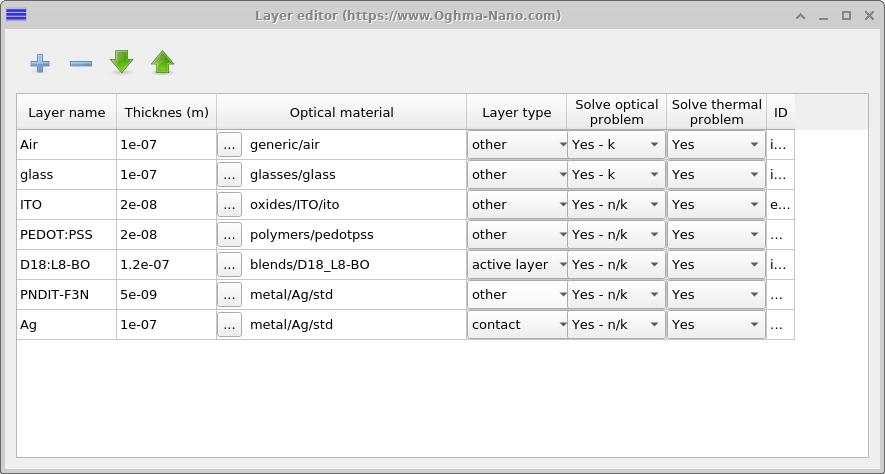
\includegraphics[width=0.8\textwidth,height=0.5\textwidth]{./images/transfer_matrix/layer_editor.png}
\caption{The layer editor showing both \emph{coherent layers} and \emph{incoherent layers}}
\label{fig:transfer_matrix_layer_editor}
\end{figure}

To get around the problem of having to simulate different length scales (problem 1) OghmaNano allows the user to set an \emph{effective} optical depth for any layer.  So one can for example setup a layer in the layer editor of width 100 nm, but set it's \emph{effective} depth to a much larger value such as 1 m. This works by multiplying the absorption coefficient of the layer by the ratio:

\begin{equation}
\alpha_{effective}(\lambda)=\alpha(\lambda) \frac{L_{effective}}{L_{simulation}}
\label{effective_depth}
\end{equation}

Where $\alpha_{effective}$ is the effective absorption used in the simulation, $\alpha$ is the true value of absorption for the material, $L_{effective}$ is the effective layer thickness (say 1 m or 1 km), and $L_{simulation}$ is the thickness of the layer in the simulation window. Not only does this approach reduce numerical issues (problem 1) but it also allows the user to plot meaningful graphs of the simulation results, without most of the plot taken up by the substrate and the device only appearing as a tiny slither on the edge of the graph.

If you want to use this feature, then set up a device structure as shown in \ref{fig:transfer_matrix_layer_editor} then in the transfer matrix window click the Optical Thickness button (top right of Figure \ref{fig:optical_thickness}). Then the window \ref{fig:optical_thickness_window} will appear. In this window you can set the \emph{effective optical thickness} of any layer. In this case we have set the glass to be 1 meter thick.

\begin{minipage}{0.5\textwidth}
	\centering
	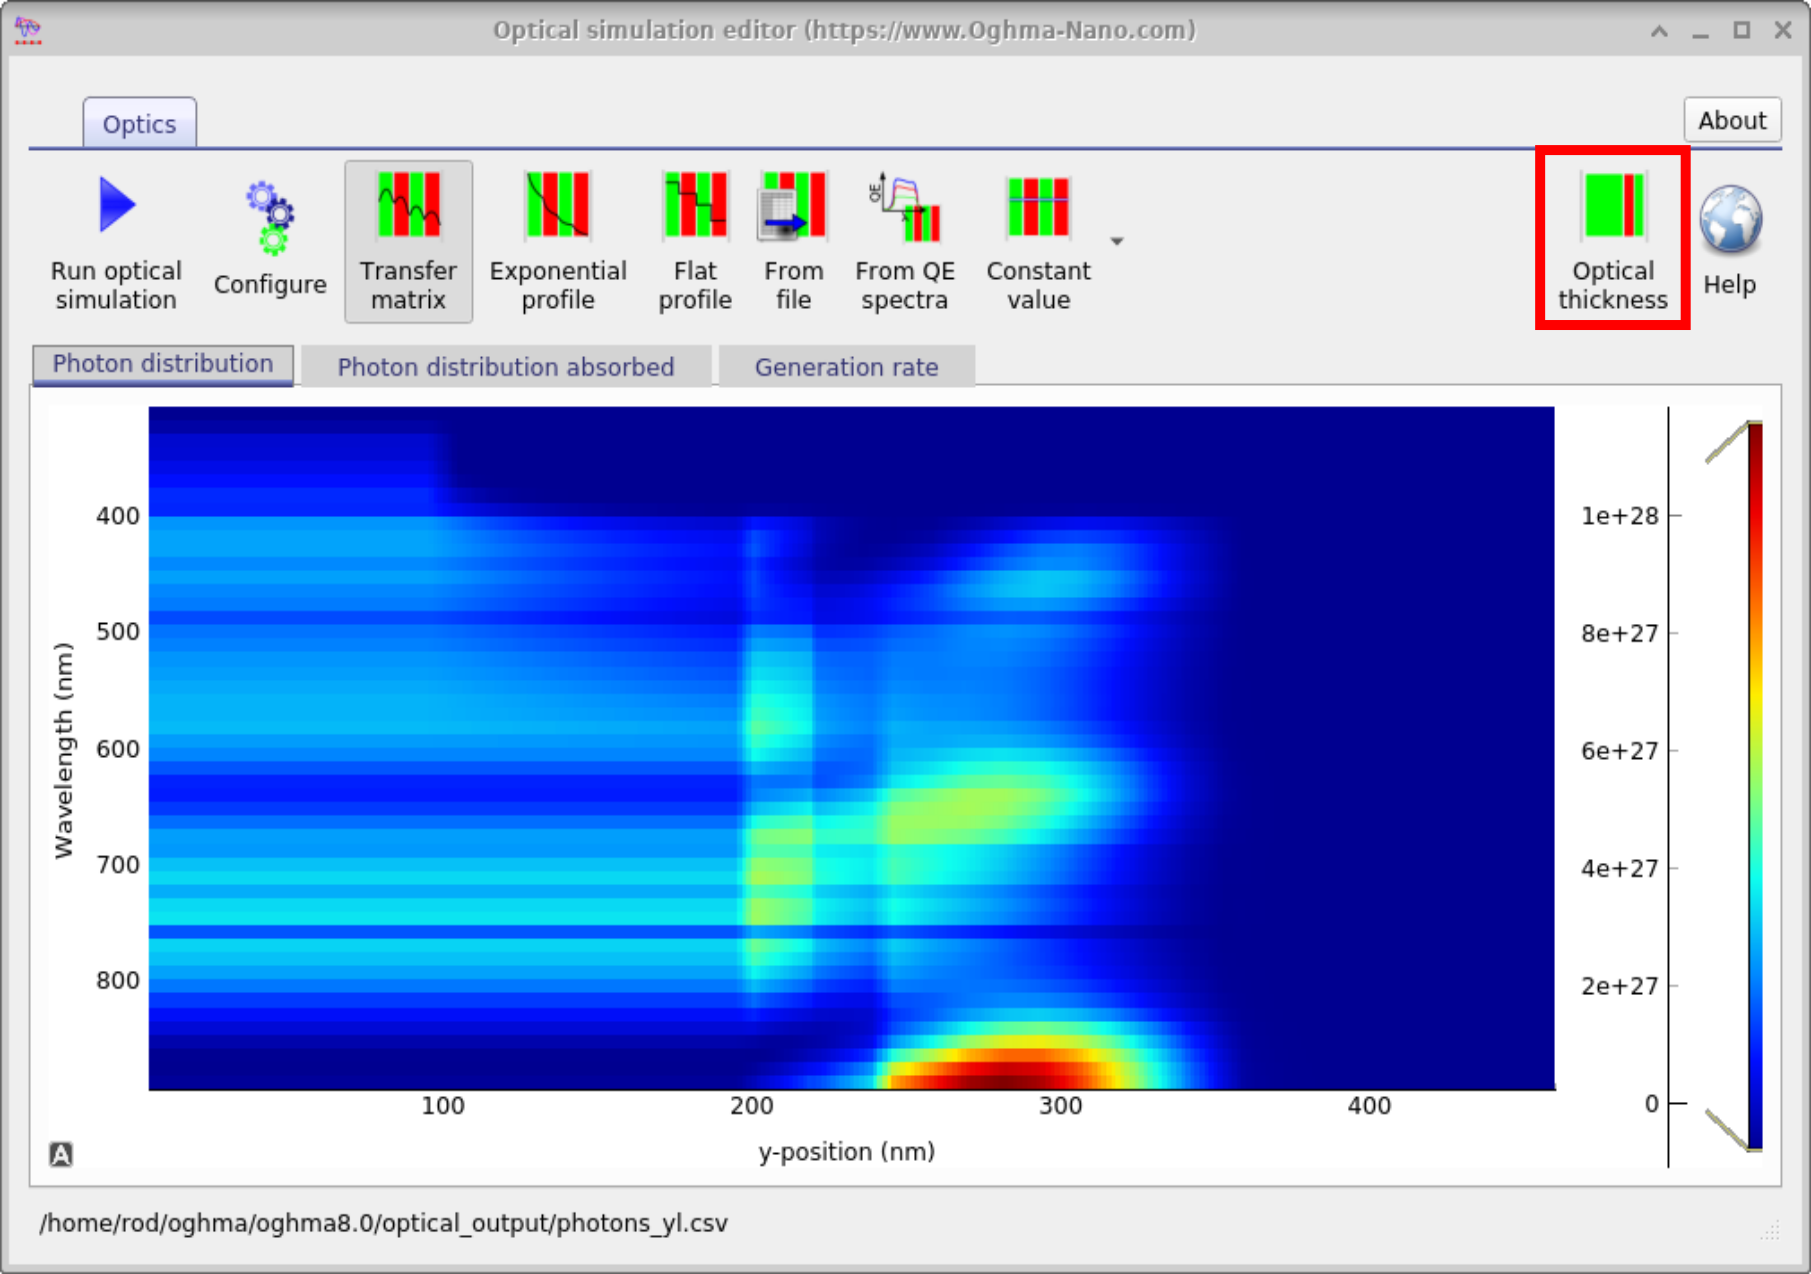
\includegraphics[width=\linewidth,height=0.8\linewidth]{./images/transfer_matrix/thickness.png}
	\captionof{figure}{Opening the effective optical thickness window.}
	\label{fig:optical_thickness}
\end{minipage}
\hspace{4pt}
\begin{minipage}[]{0.5\linewidth}
	\centering
	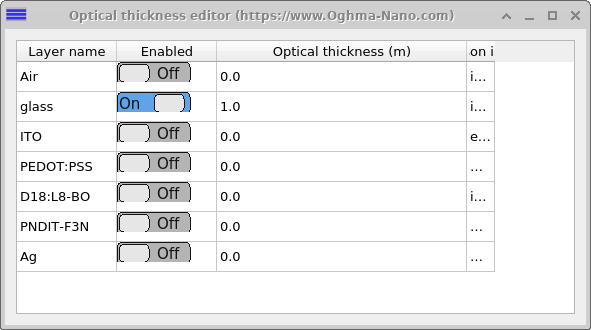
\includegraphics[width=\linewidth,height=0.6\linewidth]{./images/transfer_matrix/layer_thickness.png}
	\captionof{figure}{The effective optical thickness window, you can see that for this structure the optical thickness of glass has been set to 1 meter.}
	\label{fig:optical_thickness_window}
\end{minipage}


\pagebreak
